\documentclass[margin=small, twocolumn]{hsrzf}

\usepackage{hsrstud}

\numberwithin{equation}{subsection}

\usepackage{multicol}

\usepackage{float}
\usepackage{array}
\usepackage{booktabs}
\usepackage{rotating}
\usepackage{enumitem}

\usepackage{graphicx}
\usepackage{xcolor}

\usepackage[
    type={CC},
    modifier={by-nc-sa},
    version={4.0},
]{doclicense}


\usepackage{polyglossia}
\setdefaultlanguage[variant=swiss]{german}


\title{Analysis 2 Zusammenfassung}
\author{Naoki Pross}
\date{Fr\"uhlingsstemester 2020}


\newcommand{\brpage}[1]{\textcolor{red!70!black}{\small\texttt{S#1}}}

\begin{document}

%%%%%%%%%%%%%%%%%%%%%%%%%%%%%%%%%%%%%%%%%%%%%%%%%%%%%%%%%%%%%%%%%%%%%%%%%%%%%%%

\section{Integration \brpage{493,507}}
\subsection{Tricks \brpage{495}}
Linearit\"at \brpage{495}
\[
    \int k(u + v) = k\left(\int u + \int v\right)
\]
Partialbruchzerlegung \brpage{15,498}
\[
    \int \frac{f(x)}{P_n(x)} \di{x} = \sum_{k=1}^n \int \frac{A_k}{x-r_k}\di{x}
\]
Elementartransformation \brpage{496}
\[
    \int f(\lambda x + \ell) \di{x} = \frac{1}{\lambda} F(\lambda x + \ell) + C
\]
Partielle Integration \brpage{497}
\[
    \int u \di{v} = uv - \int v \di{u}
\]
Potenzenregel \brpage{496}
\[
    \int u^n \cdot u' = \frac{u^{n+1}}{n+1} + C \qquad n \neq -1
\]
Logaritmusregel \brpage{496}
\[
    \int \frac{u'}{u} = \ln|u| + C
\]
Allgemeine Substutution \brpage{497}\\
 \(x = g(u)\), und \(\dd{x} = g'(u)\dd{u}\)
\[
    \int f(x) \di{x} = \int (f\circ g) ~ g' \di{u} = \int \frac{f \circ g}{(g^{-1})'\circ g} \di{u} 
\]
Universalsubstitution \brpage{504}
\begin{align*}
    t &= \tan(x/2) & \sin(x) &= \frac{2t}{1+t^2} \\
    \dd{x} &= \frac{2\dd{t}}{1+t^2} & \cos(t) &= \frac{1-t^2}{1+t^2} 
\end{align*}
Womit
\[
    \int f(\sin(x), \cos(x), \tan(x)) \di{x} = \int g(t) \di{t}
\]

\subsection{Uneigentliches Integral \brpage{520}}
\begin{align*}
    \int\limits_a^\infty f \di{x} &= \lim_{B \to \infty} \int\limits_a^B f \di{x} \\
    \int\limits_{-\infty}^b f \di{x} &= \lim_{A \to -\infty} \int\limits_A^b f \di{x} \\
    \int\limits_{-\infty}^\infty f \di{x} &= \lim_{\substack{A \to +\infty \\ B \to -\infty}} \int\limits_A^B f \di{x}
\end{align*}
Wenn \(f\) im Punkt \(u \in (a,b)\) nicht definiert ist.
\begin{equation} \label{eqn:int-with-pole}
    \int\limits_a^b f \di{x} = 
    \lim_{\epsilon\to +0} \int\limits_a^{u-\epsilon} f \di{x}
    + \lim_{\delta\to +0} \int\limits_{u+\delta}^b f \di{x}
\end{equation}

\subsection{Cauchy Hauptwert \brpage{523}}
Der C.H. (oder PV f\"ur \emph{Principal Value} auf Englisch) eines uneigentlichen Integrals ist der Wert, wenn in einem Integral wie \eqref{eqn:int-with-pole} beide Grenzwerte mit der gleiche Geschwindigkeit gegen 0 streben.
\[
    \text{C.H.} \int\limits_a^b f \di{x} = 
    \lim_{\epsilon\to +0} \left( \int\limits_a^{u-\epsilon} f \di{x}
    + \int\limits_{u+\epsilon}^b f \di{x} \right)
\]
Zum Beispiel \(x^{-1}\) ist nicht \"uber \(\mathbb{R}\) integrierbar, wegen des Poles bei 0. Aber intuitiv wie die Symmetrie vorschlagt
\[
    \text{C.H.} \int\limits^\infty_{-\infty} \frac{1}{x} \di{x} = 0
\]

\subsection{Majorant-, Minorantenprinzip und Konvergenzkriterien \brpage{521,473,479,481}}

Gilt f\"ur die Funktionen \(0 < f(x) \leq g(x)\) mit \(x \in [a,\infty)\)
\[
    \text{konvergiert } \int\limits_a^\infty g \di{x} 
    \implies \text{ konvergiert } \int\limits_a^\infty f \di{x}
\]
Die selbe gilt umgekehrt f\"ur Divergenz. Wenn \(0 < h(x) \leq f(x)\) 
\[
    \text{divergiert } \int\limits_a^\infty h \di{x} 
    \implies \text{ divergiert } \int\limits_a^\infty f \di{x}
\]
\(g\) und \(h\) hei{\ss}en Majorant und Minorant bzw.

%%%%%%%%%%%%%%%%%%%%%%%%%%%%%%%%%%%%%%%%%%%%%%%%%%%%%%%%%%%%%%%%%%%%%%%%%%%%%%%

\section{Implizite Ableitung \brpage{448}}
\begin{alignat*}{3}
  (af)' &= af' &\quad&& (u(v(x)))' &= u'(v)v' \\
  (uv)' &= u'v + uv' &\quad&& \left(\frac{u}{v}\right)' &= \frac{u'v-uv'}{v^2} \\
  \left(\sum u_i\right)' &= \sum u'_i &\quad&& (\ln u)' &= \frac{u'}{u} \\
  (f^{-1})' &= \frac{1}{f'(f^{-1}(x))}
\end{alignat*}
Alle normale differenziazionsregeln f\"ur \(f(x)\) gelten.
Allgemeiner f\"ur die implizite Funktion \(F(x,y) = 0\)
\[
 	\dd{y} = y'\dd{x}
	\qquad
	\pderiv{F}{x} + \pderiv{F}{y} y' = 0
\]

%%%%%%%%%%%%%%%%%%%%%%%%%%%%%%%%%%%%%%%%%%%%%%%%%%%%%%%%%%%%%%%%%%%%%%%%%%%%%%%

\section{Differentialgeometrie}
\subsection{Ebene Kurven \brpage{250}}

\subsubsection{Darstellungen und Umwanldung}
\begin{figure}[h]
\centering
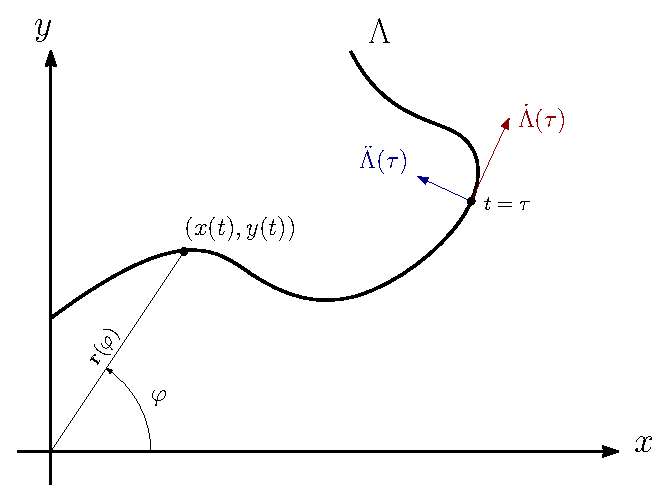
\includegraphics[width=.9\linewidth]{fig/plane-curve.eps}
\caption{Die ebene Kurve \(\vec{\Lambda}(t)\) kann Explizit \(y(x)\) (in diesem Fall nicht), Implizit \(\vec{u}(x,y) = 0\), Polar \(\vec{r}(\varphi)\) oder in Parameterform \((x(t), y(t))\) dargestellt werden.}
\label{fig:plane-curve}
\end{figure}

Sei \(\Lambda: x = \phi(t),\, y = \psi(t), t\in I\) eine glatte Jordankurve.
Beispiel in Abb. \ref{fig:plane-curve}.

\paragraph{Polar zu Kartesian}
\[
    r = \sqrt{x^2 + y^2}
    \qquad
    \tan\varphi = y/x
\]
\[
    x = r \cos\varphi
    \qquad
    y = r \sin\varphi
\]

\paragraph{Parametrisch zu explizit}
Sei \(\dot{\phi} \neq 0\) oder \(\dot{\psi} \neq 0\). Im Falle \(\dot{\phi} \neq 0\), wechselt \(\dot\phi\) in der Umgebung von \(t\) das Vorzeichen nicht, \(\phi\) ist dort streng monoton.
Daher gilt
\[
    t = \phi^{-1}(x) \quad y = \psi(t) = \psi \circ \phi^{-1}(x) = f(x)
\]
Wenn \(\dot{\psi} \neq 0\) ist dann \(x = \phi \circ \psi^{-1}(y)\)

\subsubsection{Bogenl\"ange \brpage{251,514}} \label{sec:arc-length}
Weitere Formeln (z.B. polar) findet man in Tab. \ref{tab:plane-curves-big}.
\[
    \ell = \int\limits_a^b \sqrt{1 + (f')^2} \di{x} 
    = \int\limits_{t_0}^{t_1} |\dot{\vec{c}}| \di{t}
\]

\subsubsection{Umparametrisierung nach Bogenl\"ange}
Sei die Kurve \(\vec{\Lambda}(t), t \in I\) mindestens einmal differenzierbar, und \(\ell\) die Bogenl\"ange (gem\"a{\ss} \S\ref{sec:arc-length}) im Intervall. Die Umparametrisierung \(\vec{\Lambda}(s)\) ist dann
\[
    s = \ell t \implies \vec{\Lambda}(s) = \vec{\Lambda}(t/\ell)
\]
Die neue Parametrisierung hat \(\vec{\Lambda}' = 1\) (nach \(s\) differenziert), d.h. die erste Ableitung ist der tangent Einheitsvector!

\subsubsection{Tangente und Normalvektor \brpage{251,252}}
F\"ur eine ebene Kurve \(\vec{\Lambda}(t)\) \(\tau, t \in I\), der Vektor \(\dot{\vec\Lambda}(\tau)\) ist immer an \(\vec{\Lambda}(\tau)\) tangent. \(\ddot{\vec{\Lambda}}(\tau)\) ist zur Kurve normal.
\begin{align*}
    \dot{\vec{\Lambda}}
    &= \deriv{y}{x} 
    = \frac{\dot{y}}{\dot{x}} 
    = \frac{r'\sin\varphi + r\cos\varphi}{r'\cos\varphi - r\sin\varphi}
    \\[.9em]
    \ddot{\vec{\Lambda}}
    &= \deriv[2]{y}{x}
    = \frac{\ddot{y}\dot{x} - \ddot{x}\dot{y}}{\dot{x}^3}
\end{align*}
Man kann auch die Tangentengleichung und die Normalengleichung zur Zeitpunkt \(\tau\) finden
\begin{align*}
    T: y - \psi(\tau) &= \frac{\dot{\psi}}{\dot{\phi}}(x - \phi(\tau)) \\
    N: y - \psi(\tau) &= -\frac{\dot{\phi}}{\dot{\psi}}(x - \phi(\tau))
\end{align*}

\subsubsection{Kr\"ummung und Kr\"ummungsradius \brpage{254}}
Siehe Tab. \ref{tab:plane-curves-big} f\"ur die Rechnungsformeln und Abb. \ref{fig:plane-curvature} f\"ur eine graphische Deutung.
\[
    \kappa 
    = \lim_{\Delta s\to 0} \frac{\Delta \theta}{\Delta s}
    = \deriv{\theta}{s} 
    \qquad
    R = 1/\kappa
\]
Eine gerade hat \(\kappa = 0\) und \(R = \infty\).
Entsprechend der Orientierung der \(x\)-Achse, entspricht einer \(\kappa > 0\) eine Linkskr\"ummung und \(\kappa < 0\) eine Rechtskr\"ummung.

Der Kr\"ummungskreis hat Ma{\ss}zahl \(\rho = 1/|\kappa|\) und Mittelpunkt \(P_c\) gem\"a\ss
\[
    P_c = \begin{pmatrix} x_c \\ y_c \end{pmatrix} 
    = \begin{pmatrix} x \\ y \end{pmatrix} + \frac{1}{\kappa} \vec{\hat{n}}
\]
Wobei \(\uvec{n} = \vec{\ddot{\Lambda}}^0\) ist der Normalvektor.

\subsubsection{Konvexit\"at}
Sei die Kurve \(\Lambda\) durch \(f \in C^2\) auf \([a,b]\) gegeben.
\begin{itemize}
    \item \(f\) ist auf \((a,b)\) konvex (bzw. konkav), wenn \(\kappa \geq 0\) (bzw. \(\kappa \leq 0\)) \(\forall x \in (a,b)\).
    \item \(f\) ist auf \((a,b)\) streng konvex (bzw. konkav), wenn \(\kappa > 0\) (bzw. \(\kappa < 0\)) \(\forall x \in (a,b)\).
    \item Hat in \(\Lambda\) in \(P\) einen Wendepunkt, dann \(\kappa(P) = 0\).
\end{itemize}

\subsubsection{Evoluten und Evolventen \brpage{262}}


\begin{figure}[h]
\centering
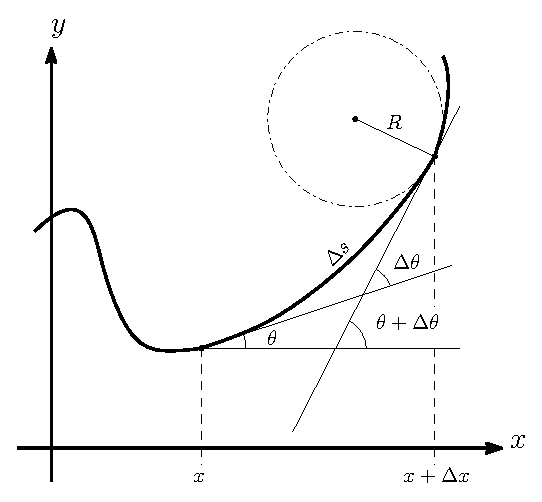
\includegraphics[width=.8\linewidth]{fig/plane-curvature}
\caption{Kr\"ummung und Kr\"ummungskreisradien}
\label{fig:plane-curvature}
\end{figure}

\subsection{Raumkurven \brpage{263}}

\subsection{Kurven 2. Ordnung -- Kegelschnitt \brpage{212}}
Die Polarform f\"ur die allgemeine Gleichung der Kurver 2. Ordnung ist
\begin{equation} \label{eqn:conics-polar}
    r = \frac{p}{1 + \varepsilon \cos\varphi}
\end{equation}
Der parameter \(\varepsilon\) \"andert die Gestalt folgendermaßen
\begin{multicols}{2}
\begin{itemize}
    \item \(\varepsilon = 0\) Kreis
    \item \(|\varepsilon| \in (0;1)\) Ellipse
\end{itemize}
\columnbreak
\begin{itemize}
    \item \(|\varepsilon| = 1\) Parabel
    \item \(|\varepsilon| > 1\) Hyperbel
\end{itemize}
\end{multicols}

\subsubsection{Kreis \brpage{204}}
{\renewcommand{\arraystretch}{1.1}
\begin{tabular}{l >{\(\displaystyle}l<{\)}}
    Kartesisch & (x - C_x)^2 + (y - C_y)^2 = r^2 \\
    Parameter  & x = c_x + R\cos t \quad y = c_y + R\sin t
\end{tabular}}

\subsubsection{Ellipse \brpage{205}}
{\renewcommand{\arraystretch}{2}
\begin{tabular}{l >{\(\displaystyle}l<{\)}}
    Kartesisch & \left(\frac{x - C_x}{a}\right)^2 + \left(\frac{y - C_y}{b}\right)^2 = 1 \\
    Parameter  & x = a\cos t \quad y = b\sin t
\end{tabular}}

\subsubsection{Hyperbel \brpage{207}}
{\renewcommand{\arraystretch}{2}
\begin{tabular}{l >{\(\displaystyle}l<{\)}}
    Kartesisch & \left(\frac{x - C_x}{a}\right)^2 - \left(\frac{y - C_y}{b}\right)^2 = 1 \\
    Parameter  & x = a\cosh t \quad y = b\sinh t
\end{tabular}}

\subsubsection{Parabel \brpage{210}}
\begin{tabular}{l >{\(\displaystyle}l<{\)}}
    Kartesisch & y = ax^2 + bx + c \\
    Parameter  & x = t \quad y = at^2 + bt + c
\end{tabular}

\subsection{Kurven 4. Ordnung \brpage{98}}
\paragraph{Kardioide / Herzkurve \brpage{99,100}}
\[
    r = a(1 + cos\varphi)
\]

\paragraph{Lemniskate \brpage{101}}
\[
    r = a \sqrt{2\cos(2\varphi)}
\]

%%%%%%%%%%%%%%%%%%%%%%%%%%%%%%%%%%%%%%%%%%%%%%%%%%%%%%%%%%%%%%%%%%%%%%%%%%%%%%%

\section{Reihen}
\subsection{Bemerkenswerte Rehien \brpage{19,477}}
\paragraph{Arithmetische Reihe}
Sei \(a_1 \in \mathbb{R}\) und \(d \in \mathbb{R} \setminus \{0\}\), dann aus der arithmetischen Folge \(\langle a_k \rangle\) mit \(a_k = a_1 + (k-1)d\) erh\"alt man die Reihe \(\langle A_n \rangle\) mit:
\begin{align*}
    A_n &= a_1 + \sum_{k=1}^n (k-1)d = a_1 + d + 2d + \cdots + (n-1)d\\
    &= \frac{n}{2}\big( 2a_1 + (n-1)d\big) = \frac{n}{2}(a_1 + a_n)
\end{align*}
    
\paragraph{Geometrische Reihe}
Sei \(a_1 \in \mathbb{R}\) und \(q \in \mathbb{R} \setminus \{0;1\}\). Aus der geometrischen Folge \(\langle g_k \rangle\) mit \(g_k = a_1 q^k\) erh\"alt man die Reihe \(\langle G_n \rangle\) mit:
\[
    G_n = a_1 \sum_{k=1}^n q^{k-1} = a_1 \frac{1-q^n}{1-q}
\]
    
\paragraph{Harmonische Reihe}
Aus der folge \(\langle h_k \rangle\) mit \(h_k = 1/k\) erh\"alt man die Reihe \(\langle H_n \rangle\) mit:
\[
    H_n = \sum_{k=1}^n = 1 + \frac{1}{2} + \frac{1}{3} + \cdots + \frac{1}{n}
\]

\paragraph{Potenzreihe} Siehe \S\ref{sec:powerseries}

\subsection{Unendlichen \brpage{470,477}}
Sei \(\langle a_n \rangle\) eine Folge die Reihe \(\langle S_n \rangle\),
\[
    S_n = \sum_{k=1}^n a_k \qquad S = \lim_{n\to\infty} S_n
\]

\subsubsection{Konvergenz \brpage{472,475}}

\paragraph{Absolute \brpage{475}}
Die Reihe \(S_n\) hei{\ss}t \emph{absoulut konvergent} wenn
\[
    \lim_{n\to\infty} \sum_{k=1}^n \left| a_k \right| \text{ konvergiert}
\]
Wenn eine Reihe absolut konvergent ist, dann
\begin{enumerate}
    \item sie ist auch konvergent.
    \item die Glieder k\"onnen nach Belieben miteinander vertauscht weden.
    \item sei \(\displaystyle 
        c_n = \sum_{k=1}^n a_k b_{n-k+1} = a_n b_1 + a_{n-1} b_2 + \cdots + a_1 b_n
    \) (\(a_n\) und \(b_n\) abs. konvergent gegen \(a\) bzw. \(b\)), dann
    \[
        \sum_{n=1}^\infty c_n = 
        \left(\sum_{n=1}^\infty a_n\right)
        \left(\sum_{n=1}^\infty b_n\right)
    \]
\end{enumerate}

\paragraph{Bedingte} Wenn die Reihe \(S_n\) nicht abs. konvergiert, aber es eine Umordnung gibt, soda{\ss} die umgeordnete Reihe entweder divergent ist oder gegen eine von verschiedene Summe konvergiert. Dann hei{\ss}t die Reihe \emph{bedingt konvergent}.


\subsubsection{Konvergenzkriterien \brpage{472}}

\paragraph{Cauchy'sches \brpage{475}}
\[
    \forall \varepsilon > 0 : \forall m,n \in \mathbb{N}, m > n:
    \left| \sum_{k=n+1}^m a_k \right| < \varepsilon
\]

\paragraph{Wurzelkriterium von Cauchy \brpage{474}}
\[
    \alpha = \limsup_{n\to\infty} \sqrt[n]{\left| a_n \right|}
    \implies\begin{cases}
        \alpha < 1 \quad \text{(abs.) konvergent} \\
        \alpha > 1 \quad \text{divergent}
    \end{cases}
\]
Wenn \(\alpha = 1\)  man kann nicht direkt eine Konvergenz / Divergenz schliessen.

\paragraph{Quotientenkriterium von d'Alambert \brpage{474}}
\[
    \alpha = \lim_{n\to\infty} \left|\frac{a_{n+1}}{a_n}\right|
    \implies\begin{cases}
        \alpha < 1 \quad \text{(abs.) konvergent} \\
        \alpha > 1 \quad \text{divergent}
    \end{cases}
\]

\paragraph{Leibniz'sches (f\"ur alternierenden Reihen) \brpage{476}}
Wenn \(\langle a_n \rangle\) eine alterniende Folge ist, dann gilt
\begin{gather*}
    \langle |a_n| \rangle \text{ ist eine monoton fallende Nullfolge} \\
    \implies \langle s_n \rangle \text{ konvergiert}
\end{gather*}

\paragraph{Integralkriterium \brpage{475}}
Sei \(f(x) \geq 0\), \(x \in [1;\infty)\) und \(f\downarrow\). Merkt man dass:
\[
    \overbrace{\int\limits_1^n f(x) \dd{x}}^{S} 
    \leq \sum_{k=1}^n a_k
    \leq \overbrace{\int\limits_2^n f(x-1) \dd{x}}^{\text{Auch } S}
\]
Somit folgt:
\[
    \text{konvergiert } \int\limits_1^\infty f(x) \dd{x}
    \implies \text{konvergiert } s
\]

\subsection{Potenzreihen \brpage{482}} \label{sec:powerseries}
\begin{align*}
    P &= \sum_{n=0}^\infty a_n (x - x_0)^n \\
      &= a_0 + a_1 (x - x_0) + a_2 (x - x_0)^2 + \cdots
\end{align*}
Sei \(\lim_{n\to\infty} \sqrt{|a_n|} = a \) (Wurzelkriterium)
\begin{align*}
    a = 0 &\implies \text{ abs. konvergent} \\
    a > 0 &\implies
    \forall x \in \mathbb{R}:
    \begin{cases}
        |x| < 1/a: \text{ abs. konvergent} \\
        |x| > 1/a: \text{ divergent}
    \end{cases}
\end{align*}

\subsubsection{Konvergenzradius/-bereich \brpage{482}}
Sei \(\langle \sqrt{|a_n|}\rangle\) nicht beschr\"ankt (\(a = \infty\)), so ist \(P\) nur f\"ur \(x=x_0\) konvergent (\(r = 1/\infty = 0^+\)). Sonst existiert der \emph{Konvergenzradius} \(r \in\mathbb{R}^+\):
\begin{align*}
    r &= \limsup_{n\to\infty} \left| \frac{a_n}{a_{n+1}} \right| &
    r &= \left( \limsup_{n\to\infty} \sqrt[n]{| a_n |} \right)^{-1}
\end{align*}
Innerhalb des \emph{Konvergenzbereiches} \(\{ x : |x - x_0| < r\} = (x_0-r; x_0+r)\) ist die Reihe absolut konvergent, ausserhalb dessen ist sie divergent.
Wenn \(r = \infty\) dann ist die Reihe abs. konvergent.

\subsubsection{Funktion darstellen}

\subsubsection{Ableitung und Integration}
Sei \(P\) eine Potenzreihe mit dem Konvergenzradius \(r > 0\), die eine Funktion \(f\) darstellt. Innerhalb des Konvergenzradius gilt:
\begin{align*}
    f'(x) &= \left(\sum_{n=0}^\infty a_n x^n \right)' 
        = \sum_{n=1}^\infty n a_n x^{n-1} \\
    \int f \di{x} &= \int \sum_{n=0}^\infty a_n x^n \di{x}
        = \sum_{n=0}^\infty \frac{a_n}{n+1} x^{n+1} + C
\end{align*}
H\"ohere Ableitungen:
\[
    f^{(k)}(x) = \left(\sum_{n=0}^\infty a_n x^n \right)^{(k)} 
    = \sum_{n=k}^\infty \frac{n!}{(n-k)!} a_n x^{n-k}
\]

\subsubsection{Taylor Polynom und Reihe \brpage{484}}
Der Taylor-Polynom approximiert eine Funktion um einen Entwicklungspunkt \(a\).
\begin{align*}
  T_n(x, a) &= \sum_{k=0}^n\frac{f^{(k)}(a)}{k!}(x-a)^k + R_n\\
  &= f(a) + \frac{f'(a)}{1!}(x-a)^1 + \frac{f''(a)}{2!}(x-a)^2 + \cdots
\end{align*}
Die Restgliede sind
\begin{align*}
  R_n = \frac{f^{(n+1)}(\xi)}{(n+1)!} (x-a)^{(n+1)} \qquad (\xi \in (x;a))
\end{align*}
Wenn \(\lim_{n\to\infty}R_n = 0\) dann \(f(x) = T(x,a)\), d.h. die Taylor Rehie zu \(f\) identisch ist (Konvergenzradius \(r = \infty\)). Sonst berechnet man der \emph{worst case} Fehler \(\epsilon \geq |R_n|\) und der dazugeh\"orig \(\hat{\xi} = \underset{\xi}{\arg}\max|R_n|\):
\begin{align*}
  \epsilon
  = \max |R_n|
  = \max \left[\frac{|f^{(n+1)}(\xi)|}{(n+1)!} |x-a|^{(n+1)}\right]
\end{align*}

%%%%%%%%%%%%%%%%%%%%%%%%%%%%%%%%%%%%%%%%%%%%%%%%%%%%%%%%%%%%%%%%%%%%%%%%%%%%%%%

\section{Differentialgleichungen}
\subsection{Definition}
Eine Funktion \(y = \varphi(x)\) hei{\ss}t \emph{allgemeine} L\"osung der \(n\)-te Ordnung Differentialgleichung
\[
    F(x, y, y', y'', \dots, y^{(n)}) = 0
\]
auf dem Intervall \(I\), wenn
\begin{itemize}
    \item \(\varphi\) auf \(I\) \(n\)-mal differenzierbar ist
    \item \(\forall x \in I: F(x, \varphi, \varphi', \varphi'', \dots, \varphi^{(n)}) = 0\)
\end{itemize}

Gegeben seien auch der \emph{Anfangspunkt}
\(x_0\), und
die \emph{Anfangswerte} oder \emph{Anfangsbedingungen}
\(y_0 = y(x_0)\),
\(y_1 = y'(x_0)\),
\dots,
\(y_{n-1} = y^{(n-1)}(x_0) \in \mathbb{R}\).
Dann hat man ein \emph{Anfangswertproblem}, der eine \emph{spezifische} L\"osung ergibt.

\subsection{DGL 1. Ordnung}
Die funktionen \(f\) und \(g\) seien auf demselben Intervall \(I\) stetig. Die Differentialgleichung
\[
    y' + f(x)y = g(x)
\]
hei{\ss}t \emph{homogen}, wenn \(g\) die Nullfunktion (\(=0\)) auf \(I\) ist, sonst \emph{inhomogen}. \(g\) hei{\ss}t St\"orglied.

\paragraph{Separation} Wenn die DGL die Form \(y' = g(y) f(x)\) hat, dann l\"asst sie sich mit der Umformung
\begin{gather*}
    \frac{y'}{g(y)} = f(x) \implies \int \frac{\dd{y}}{g(y)} = \int f(x) \di{x} \\
\end{gather*}
Ein Speziallfall \(g(y) = y\) hat die allgemeine L\"osung
\[
    y = k\exp\left(\int f(x) \di{x} \right) = k \nemathit{e}^{F}
\]

\paragraph{Substitution Linearterm} Hat die DGL die Form \(y' = f(ax + by + c)\), dann benutzt man die Substitution
\begin{align*}
    z  &= ax + by + c \iff y(z) = b(z-c)/ax \\
    z' &= a + by' \implies z' = a + b y'(z) \text{ separiert!}
\end{align*}
Dann soll sie nach \(z\) l\"osen lassen.

\paragraph{Glaichgradigkeit} Hat die DGL die Form \(y' = f(y/x) \quad x \neq 0\), dann benutzt die Substitution
\begin{align*}
    z = y/x &\implies y' = z'x + z \\
    &\implies z' = \frac{1}{x}\left(y'(x) - z\right) \quad\text{separiert!}
\end{align*}

\subsection{DGL 2. Ordnung}


\begin{thebibliography}{3}
  \bibitem{hsr}
    \texttt{An2E} Vorlesungen an der Hochschule f\"ur Technik Rapperswil und der dazugeh\"orige Skript,
    \textit{Dr. Bernhard Zgraggen}, Fr\"uhlingssemester 2020
  \bibitem{bronstein}
    Taschenbuch der Mathematik,
    10. \"uberarbeitete Auflage, 2016 (1977),
    \textit{Bronstein, Semendjajew, Musiol, M\"uhlig}, 
    \texttt{ISBN 978-3-8085-5789-1}
  \bibitem{mathe2}
    Mathematik 2: Lehrbuch für ingenieurwissenschaftliche Studieng\"ange,
    2012, 7. Auflage, XII, Springer Berlin,
    \textit{Albert Fetzer, Heiner Fränkel},
    \texttt{ISBN-10 364224114X},
    \texttt{ISBN-13 9783642241147}
    
\end{thebibliography}

\section*{Notation}
Rot markierte Zahlen wie zB \brpage{477} sind Hinweise auf die Seiten im ``Bronstein'' \cite{bronstein}

\begin{itemize}
    \item \(C^n\) ist der Menge der glatten \(n\)-mal differenzierb\"aren Funktionen.
    \item Das Zeichen \(\forall\) bedeutet ``f\"ur alle''
\end{itemize}

\section*{License}
{ \tt
An2E-ZF (c) by Naoki Pross
\\\\
An2E-ZF is licensed under a Creative Commons Attribution-ShareAlike 4.0 Unported License.
\\\\
You should have received a copy of the license along with this work. If not, see 
\\\\
{\small\url{http://creativecommons.org/licenses/by-sa/4.0/}}
}


\onecolumn

\begin{sidewaystable}[p]
\centering
\caption{Rechnungen bez. ebene Kurven}
\label{tab:plane-curves-big}
\renewcommand{\arraystretch}{3}
\begin{tabular}{l *{3}{>{\(\displaystyle}l<{\)}} }
\toprule
\textbf{Ebene Kurven} & \textbf{Kartesich } y = f(x) & \textbf{Polar } \vec{r}(\varphi) & \textbf{Parameter } \vec{c}(t) = \left(x(t), y(y)\right) \\
\midrule
Anstieg \brpage{448}
    & f'
    & \frac{r'\sin\varphi + r\cos\varphi}{r'\cos\varphi - r\sin\varphi}
    & \dot{x}/\dot{y}
\\
Fl\"ache \brpage{493}
    & \int\limits_a^b |f(x)| \di{x}
    & \frac{1}{2}\int\limits_\alpha^\beta r(\varphi)^2 \di{\varphi}
    & \frac{1}{2}\int\limits_{t_0}^{t_1} x\dot{y} - \dot{x}y \di{t} = \frac{1}{2}\int\limits_{t_0}^{t_1}\det(\vec{c},\dot{\vec{c}}) \di{t}
\\
Bogenl\"ange \brpage{251,514}
    & \int\limits_a^b \sqrt{1 + (f')^2} \di{x}
    & \int\limits_\alpha^\beta \sqrt{(r')^2 + r^2} \di{\varphi}
    & \int\limits_{t_0}^{t_1} \sqrt{\dot{x}^2 + \dot{y}^2} \di{t} = \int\limits_{t_0}^{t_1} |\dot{\vec{c}}| \di{t}
\\
Kr\"ummung \(\kappa\) \brpage{254}
    & \frac{f''}{\sqrt{1+(f')^2}^3}
    & \frac{2(r')^2 - r r'' + r^2}{\sqrt{r^2 + (r')^2}^3}
    & \frac{\ddot{y}\dot{x} - \ddot{x}\dot{y}}{\sqrt{\dot{x}^2 + \dot{y}^2}^3} 
    = \frac{\det(\dot{\vec{c}},\ddot{\vec{c}})}{|\dot{\vec{c}}|^3}
\\[1em]
\midrule
Rotationsvolumen um \(x\) \brpage{516}
    & \pi \left|\int\limits_a^b y^2 \di{x} \right|
    & \pi \left|\int\limits_{t_0}^{t_1} y \dot{x} \di{t} \right|
    & \pi \left|\int\limits_\alpha^\beta r^2 \sin^2 \varphi (r'\cos\varphi - r\sin\varphi) \di{\varphi} \right|
\\
Rotationsoberfl\"ache um \(x\) \brpage{515}
    & 2\pi \int\limits_a^b |y| \sqrt{1 + (y')^2} \di{x}
    & 2\pi \int\limits_\alpha^\beta |r\sin(\varphi)| \sqrt{(r')^2 + r^2} \di{\varphi}
    & 2\pi \int\limits_{t_0}^{t_1} |y| \sqrt{\dot{x}^2 + \dot{y}^2} \di{t}
\\
% Rotationsvolumen um \(y\) \\
% Rotationsoberfl\"ache um \(y\) \\
\bottomrule
\end{tabular}
\end{sidewaystable}

\end{document}
